\documentclass[10.5pt]{beamer}
\usepackage[utf8]{inputenc}
\usetheme{PaloAlto}
%\usetheme{Madrid}
\usepackage[spanish]{babel}
\usepackage[T1]{fontenc}
\usepackage{amsmath}
\usepackage{amsfonts}
\usepackage{amssymb}
\usepackage{graphicx}
\usepackage{setspace}
\usepackage{ragged2e}
\usepackage{listings}
\usepackage{threeparttable}
\usepackage{array}
\title{Evaluadores y NURBS}
\author{Integrantes:Balboa Palma, Merly Mirano Mitchell Vasquez Sebastian}

\logo{
\includegraphics[scale=0.071]{figura/unmsm.png}}
\institute{UNMSM--Computación Cientfica}
 %\date{August 2022}
\date{\today}
%%%%%%%%%%%%%%%%%%%%%%%%%%%%%%%%%%%%%%%%%%%%%%%%%%%%%%%%%%%%%%%%%%%%%%%%%%%%%%%%%%%%%%%%%%%%%%
\begin{document}

\begin{frame}
\maketitle
\end{frame}


\begin{frame}{Contenido}
    %\small
    \tableofcontents
\end{frame}


\section{Introducción}

\begin{frame}{Introducción}
\begin{itemize}
\justifying
    \item  Las curvas y superficies suaves se dibujan aproximándolas con grandes o pequeños segmentos de línea o polígonos.
    \item   Muchas curvas y superficies pueden describirse matemáticamente mediante un pequeño número de parámetros.
    \item   Guardar 16 puntos de control para una superficie requiere menos almacenamiento que guardar 1000 triángulos junto con la información del vector normal en cada vértice. Además, sólo se aproximan a la superficie real, pero los puntos de control describen con precisión.
\end{itemize}
\end{frame}
%%%%%%%%%%%%%%%%%%%%%%%%%%%%%%%%%%%%%%%%%%%%%%%%%%%%%%%%%%%%%%%%%%%%%%%%%%%%%%%%%%%%%%%%%%%%%%%%%%
\begin{frame}{Introducción}
\begin{itemize}
\justifying
    \item  Si se quiere usar evaluadores para dibujar curvas y superficies utilizando otras bases, debemos convertir su base en una base de Bézier.
    \item   Cuando se renderiza una superficie Bézier o parte de ella utilizando evaluadores, es necesario especificar el nivel de detalle de su subdivisión.
\end{itemize}
\end{frame}
%%%%%%%%%%%%%%%%%%%%%%%%%%%%%%%%%%%%%%%%%%%%%%%%%%%%%%%%%%%%%%%%%%%%%%%%%%%%%%%%%%%%%%%%%%%%%%%%%%
\section{Evaluadores}

\begin{frame}{Evaluadores}
\begin{itemize}
\justifying
    \item Los evaluadores proporcionan una forma de especificar puntos en una curva o superficie utilizando puntos de control.
    \item   La curva o superficie puede ser renderizada con cualquier precisión. Además, los vectores normales pueden ser calculados automáticamente para las superficies.
    \item  Los puntos generados por un evaluador pueden utilizarse de muchas maneras: Para dibujar puntos donde estaría la superficie, una versión alámbrica de la superficie y una superficie completamente iluminada, sombreada e incluso texturizada.
\end{itemize}
\end{frame}

%%%%%%%%%%%%%%%%%%%%%%%%%%%%%%%%%%%%%%%%%%%%%%%%%%%%%%%%%%%%%%%%%%%%%%%%%%%%%%%%%%%%%%%%%%%%%%%%%%
\begin{frame}{Evaluadores}
\begin{itemize}
\justifying
    \item Se utilizan evaluadores para describir cualquier polinomio o splines polinómicos racionales o superficies de cualquier grado, incluye las B-splines, las NURBS (Non-Uniform Rational B-Spline), curvas y superficies Bézier y splines Hermite.

     \item   La función NURBS de la GLU es una interfaz de alto nivel: Los procesos NURBS encapsulan gran cantidad de código complejo. Gran parte del renderizado final se realiza con el evaluador, pero para ciertas condiciones (por ejemplo, recorte de curvas), los procesos NURBS utilizan polígonos planos para el renderizado.
\end{itemize}
\end{frame}
%%%%%%%%%%%%%%%%%%%%%%%%%%%%%%%%%%%%%%%%%%%%%%%%%%%%%%%%%%%%%%%%%%%%%%%%%%%%%%%%%%%%%%%%%%%%%%%%%%
\begin{frame}{Evaluadores}
\justifying
 Una curva de Bézier es una función vectorial de una variable
 \begin{block}
 \small
      \begin{equation*}
         C\left(u\right)=[X\left(u\right)Y\left(u\right)Z\left(u\right)]
      \end{equation*}
 \end{block}

Donde $u$ varía en un dominio $[0,1]$. Una superficie de Bézier es una función vectorial de dos variables.

\begin{block}
 \small
    \begin{equation*}
    S\left(u,v\right)=[X\left(u,v\right)Y\left(u,v\right)Z\left(u,v\right)]
    \end{equation*}
\end{block}

Donde $u$ y $v$ pueden variar en algún dominio. \newline

El rango puede tener una salida tridimensional, bidimensional para curvas en un plano o coordenadas de textura,o una salida cuatridimensional para especificar información RGBA.
\end{frame}
%%%%%%%%%%%%%%%%%%%%%%%%%%%%%%%%%%%%%%%%%%%%%%%%%%%%%%%%%%%%%%%%%%%%%%%%%%%%%%%%%%%%%%%%%%%%%%%%%%
\begin{frame}{Evaluadores}
\begin{block}
\justifying
    Para utilizar un evaluador, primero hay que definir la función \textbf{C()} o \textbf{S()}, habilitarla y luego utilizar el comando \textbf{glEvalCoord1()} o \textbf{glEvalCoord2()} en lugar de \textbf{glVertex*()}.
\end{block}

\begin{itemize}
\justifying

    \item Los vértices de la curva o de la superficie pueden utilizarse como cualquier otro vértice, para formar puntos o líneas. Además, otros comandos generan automáticamente series de vértices que producen una malla regular uniformemente espaciada en u (o en u y v).
\end{itemize}
\end{frame}
%%%%%%%%%%%%%%%%%%%%%%%%%%%%%%%%%%%%%%%%%%%%%%%%%%%%%%%%%%%%%%%%%%%%%%%%%%%%%%%%%%%%%%%%%%%%%%%%%%
\subsection{Evaluadores unidimensionales}

\begin{frame}{Evaluadores unidimensionales}
\begin{block}{Ejemplo 1.}
Dibuja una curva cúbica de Bézier usando cuatro puntos de control, como se muestra en la Figura 1.
\end{block}

\begin{figure}[h]
	\centering
	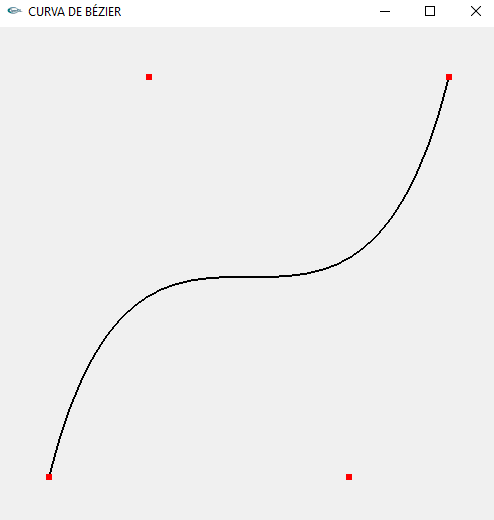
\includegraphics[width=0.5\linewidth]{figura/CURVA.PNG}
	\caption{Curva de Bézier.}
	\label{fig:propuesta}
\end{figure}

\end{frame}
%%%%%%%%%%%%%%%%%%%%%%%%%%%%%%%%%%%%%%%%%%%%%%%%%%%%%%%%%%%%%%%%%%%%%%%%%%%%%%%%%%%%%%%%%%%%%%%%%%
\subsection{Ejemplo}
\begin{frame}[fragile]
\justifying
\frametitle{Código}
La curva cúbica de Bézier se describe mediante cuatro puntos de control.
\begin{alertblock}{}
\small
\begin{verbatim}
GLfloat ctrlpoints[4][3] =
            {{-4.0, -4.0, 0.0}, { -2.0, 4.0, 0.0},
            {2.0, -4.0, 0.0}, {4.0, 4.0, 0.0}};
void init(void){
       glClearColor(0.94, 0.94, 0.94, 0.0);
       glShadeModel(GL_FLAT);
       glMap1f(GL_MAP1_VERTEX_3, 0.0, 1.0, 3, 4,
                            &ctrlpoints[0][0]);
       glEnable(GL_MAP1_VERTEX_3);
 }
\end{verbatim}
\end{alertblock}
La matriz \textbf{ctrlpoints[][]} es uno de los argumentos de \textbf{glMap1f()} y \textbf{glEnable()} habilita el evaluador unidimensional para vértices tridimensionales.
\end{frame}
%%%%%%%%%%%%%%%%%%%%%%%%%%%%%%%%%%%%%%%%%%%%%%%%%%%%%%%%%%%%%%%%%%%%%%%%%%%%%%%%%%%%%%%%%%%%%%%%%%
\begin{frame}[fragile]
\frametitle{Código}
La curva se dibuja en la rutina \textbf{display()} entre las llamadas \textbf{glBegin()} y \textbf{glEnd()}.

\begin{alertblock}{}
\small
\begin{verbatim}
    glColor3f(0.0, 0.0, 0.0);
    glBegin(GL_LINE_STRIP);
       for (int i = 0; i <= 30; i++)
           glEvalCoord1f((GLfloat) i/30.0);
    glEnd();
    glPointSize(6.0);
    glColor3f(1.0, 0.0, 0.0);
    glBegin(GL_POINTS);
        for (int i = 0; i < 4; i++)
           glVertex3fv(&ctrlpoints[i][0]);
    glEnd();
\end{verbatim}
\end{alertblock}
El comando \textbf{glEvalCoord1f()} es como emitir un \textbf{glVertex()} con las coordenadas de un vértice de la curva correspondiente al parámetro de entrada $u$.
\end{frame}
%%%%%%%%%%%%%%%%%%%%%%%%%%%%%%%%%%%%%%%%%%%%%%%%%%%%%%%%%%%%%%%%%%%%%%%%%%%%%%%%%%%%%%%%%%%%%%%%%%
\subsection{Definición y evaluación de un evaluador unidimensional}

\begin{frame}{Definición y evaluación de un evaluador unidimensional}
\justifying

El polinomio de Bernstein de grado n (u orden $n+1$ ) es dado por:
\begin{block}
\small
    \begin{equation*}
    B_i^n\left(u\right)=\left(\begin{matrix}n\\i\\\end{matrix}\right)u^i\left(1-u\right)^{n-i}
    \end{equation*}
\end{block}
Si $Pi$ representa un conjunto de puntos de control (unidimensionales, bidimensionales, tridimensionales o cuatridimensionales), entonces la ecuación:
\begin{block}
\small
    \begin{equation*}
   C\left(u\right)=\sum_{i=0}^{n}{B_i^n\left(u\right)}P_i
    \end{equation*}
\end{block}
Donde $B_{i}^{n}(u)$ son elementos de la distribución binomial respecto a $u$ y los $P_{i}$ son valores de la función que queremos aproximar.
\end{frame}
%%%%%%%%%%%%%%%%%%%%%%%%%%%%%%%%%%%%%%%%%%%%%%%%%%%%%%%%%%%%%%%%%%%%%%%%%%%%%%%%%%%%%%%%%%%%%%%%%%%%%
\begin{frame}{Definición y evaluación de un evaluador unidimensional}
\begin{itemize}
    \item Representa una curva de Bézier cuando $u$ varía de 0 a 1.
    \item Para representar la misma curva, pero permitiendo que, $u$ varíe entre $u1$ y $u2$ en lugar de 0 y 1, evaluamos:
    \begin{block}
     \small
    \begin{equation*}
          C\left(\frac{u-u_1}{u_2-u_1}\right)
    \end{equation*}
\end{block}
\end{itemize}
El comando \textbf{glMap1()} define un evaluador unidimensional que utiliza estas ecuaciones.\newline


\end{frame}

%%%%%%%%%%%%%%%%%%%%%%%%%%%%%%%%%%%%%%%%%%%%%%%%%%%%%%%%%%%%%%%%%%%%%%%%%%%%%%%%%%%%%%%%%%%%%%%%%%%%%
\begin{frame}{Definición y evaluación de un evaluador unidimensional}

   \begin{alertblock}{Comando}
   \small
    \textbf{glMap1\{fd\}} (GLenum target, TYPE u1, TYPE u2, GLint stride,
     GLint order, const TYPE *points);
   \end{alertblock}

   \begin{itemize}
   \justifying
       \item \textbf{GLenum target:} Especifica lo que representan los puntos de control, por lo tanto cuántos valores deben ser suministrados en puntos. Los puntos pueden representar vértices, datos de color RGBA, vectores normales o coordenadas de textura.

       \item \textbf{TYPE u1 y TYPE u2:} u1 y u2, indican el rango de la variable u.

       \item \textbf{GLint stride:} Es el número de valores de precisión simple o doble (según el caso) en cada bloque de almacenamiento. Por lo tanto, es un valor de desplazamiento entre el comienzo de un punto de control y el comienzo del siguiente.
   \end{itemize}

\end{frame}
%%%%%%%%%%%%%%%%%%%%%%%%%%%%%%%%%%%%%%%%%%%%%%%%%%%%%%%%%%%%%%%%%%%%%%%%%%%%%%%%%%%%%%%%%%%%%%%%%%%%%
\begin{frame}{Definición y evaluación de un evaluador unidimensional}

   \begin{alertblock}{Comando}
   \small
    \textbf{glMap1\{fd\}} (GLenum target, TYPE u1, TYPE u2, GLint stride,
     GLint order, const TYPE *points);
   \end{alertblock}

   \begin{itemize}
     \justifying
       \item \textbf{ GLint order:} El orden es el grado más uno, y debe coincidir con el número de puntos de control.

       \item \textbf{ const TYPE *points:} Los puntos apuntan a la primera coordenada del primer punto de control.
   \end{itemize}
  Utilizando la estructura de datos de ejemplo para glMap1*(), utilice lo siguiente para los puntos:
    \begin{alertblock}{}
   \small
   \begin{equation*}
       (GLfloat *) (\&ctrlpoints[0].x)
   \end{equation*}
   \end{alertblock}
\end{frame}
%%%%%%%%%%%%%%%%%%%%%%%%%%%%%%%%%%%%%%%%%%%%%%%%%%%%%%%%%%%%%%%%%%%%%%%%%%%%%%%%%%%%%%%%%%%%%%%%%%%%%
\begin{frame}{Definición y evaluación de un evaluador unidimensional}
\justifying
Se utilizan los valores de los parámetros listados en la Tabla 1 para activar cada evaluador definido antes de invocarlo.

\begin{table}[ht]
\caption{Tipos de puntos de control para \textbf{glMap1*()}.}\\
\resizebox{10cm}{!} {
\begin{center}
\begin{tabular}{ |c | c | }
\hline \textbf{Parámetro } & \textbf{Significado} \\ \hline
\justifying
GL\_MAP1\_VERTEX\_3 & coordenadas de los vértices x, y, z.\\ \hline

GL\_MAP1\_VERTEX\_4 & coordenadas de los vértices x, y, z, w. \\ \hline

GL\_MAP1\_INDEX & índice de color. \\ \hline

GL\_MAP1\_COLOR\_4 & R, G, B, A. \\ \hline

GL\_MAP1\_NORMAL & coordenadas normales. \\ \hline

GL\_MAP1\_TEXTURE\_COORD\_1 & s coordenadas de textura. \\ \hline

GL\_MAP1\_TEXTURE\_COORD\_2 & s, t coordenadas de textura. \\ \hline

GL\_MAP1\_TEXTURE\_COORD\_3  & s, t, r coordenadas de textura \\ \hline

GL\_MAP1\_TEXTURE\_COORD\_4  & s, t, r, q coordenadas de textura. \\ \hline
\end{tabular}
\end{center}}
\end{table}
 Pasamos el valor apropiado a \textbf{glEnable()} o \textbf{glDisable()} para activar o desactivar el evaluador.
\end{frame}

%%%%%%%%%%%%%%%%%%%%%%%%%%%%%%%%%%%%%%%%%%%%%%%%%%%%%%%%%%%%%%%%%%%%%%%%%%%%%%%%%%%%%%%%%%%%%%%%%%%%%
\begin{frame}[fragile]
 \frametitle{Definición y evaluación de un evaluador unidimensional}
 \justifying
\begin{itemize}
\justifying
    \item Se puede evaluar más de un evaluador a la vez. Si el evaluador GL\_MAP1\_VERTEX\_3 y  GL\_MAP1\_COLOR\_4 son definidos y habilitados, entonces \textbf{glEvalCoord1()} generan una posición como un color.

    \item Si se define y activa más de un evaluador del mismo tipo, se utiliza el de mayor dimensión.

    \item Utilizamos \textbf{glEvalCoord1*()} para evaluar un mapa unidimensional definido y habilitado.
\end{itemize}

\begin{alertblock}{}
\small
\begin{verbatim}
          void glEvalCoord1{fd} (TYPE u);
          void glEvalCoord1{fd} v (TYPE *u);
\end{verbatim}
\end{alertblock}

 Provoca la evaluación de mapas unidimensionales habilitados. El argumento $u$ es el valor (o un puntero al valor, en la versión vectorial del comando) de la coordenada del dominio.
\end{frame}
%%%%%%%%%%%%%%%%%%%%%%%%%%%%%%%%%%%%%%%%%%%%%%%%%%%%%%%%%%%%%%%%%%%%%%%%%%%%%%%%%%%%%%%%%%%%%%%%%%%%%
\subsection{Definición de valores de coordenadas uniformes en una dimensión}

\begin{frame}[fragile]
 \frametitle{Definición de valores de coordenadas uniformes en una dimensión}

\begin{itemize}
\justifying
    \item Se puede utilizar \textbf{glEvalCoord1()} con cualquier valor para $u$, pero el uso más común es con valores espaciados uniformemente, como se muestra en el Ejemplo 1.

    \item Para obtener valores uniformemente espaciados, definimos una unidimensional usando \textbf{glMapGrid1*()} y aplícamos usando \textbf{glEvalMesh1()}.
\end{itemize}

\begin{alertblock}{}
\small
\begin{verbatim}
    void glMapGrid1{fd} (GLint n, TYPE u1, TYPE u2);
\end{verbatim}
\end{alertblock}
Define una cuadrícula que va de $u1$ a $u2$ en $n$ pasos, que están espaciados uniformemente.
\begin{alertblock}{}
\small
\begin{verbatim}
    void glEvalMesh1(GLenum mode, GLint p1, GLint p2);
\end{verbatim}
\end{alertblock}
\end{frame}

%%%%%%%%%%%%%%%%%%%%%%%%%%%%%%%%%%%%%%%%%%%%%%%%%%%%%%%%%%%%%%%%%%%%%%%%%%%%%%%%%%%%%%%%%%%%%%%%%%%%%
\subsection{Definición de valores de coordenadas uniformes en una dimensión}

\begin{frame}[fragile]
 \frametitle{Definición de valores de coordenadas uniformes en una dimensión}

\begin{itemize}
\justifying
    \item Aplica la cuadrícula de mapa definida actualmente a todos los evaluadores habilitados. El modo puede ser \textbf{GL\_POINT o GL\_LINE}, dependiendo de si desea dibujar puntos o una línea conectada a lo largo de la curva.

    \item  Tiene exactamente el mismo efecto que emitir una \textbf{glEvalCoord1()} para cada uno de los pasos, incluyendo $p1$ y $p2$, donde $0\le\ p1,\ p2\le\ n$. Es equivalente a lo siguiente:
\end{itemize}

\begin{alertblock}{}
\small
\begin{verbatim}
  glBegin(GL_POINTS); /* o glBegin(GL_LINE_STRIP);*/
      for (i = p1; i <= p2; i++)
          glEvalCoord1(u1 + i*(u2-u1)/n);
  glEnd();
\end{verbatim}
\end{alertblock}
Excepto si \textbf{i = 0} o \textbf{i = n}, entonces se llama a \textbf{glEvalCoord1()} con exactamente $u1$ o $u2$ como parámetro.
\end{frame}
%%%%%%%%%%%%%%%%%%%%%%%%%%%%%%%%%%%%%%%%%%%%%%%%%%%%%%%%%%%%%%%%%%%%%%%%%%%%%%%%%%%%%%%%%%%%%%%%%%%%%
\end{document}
